\subsection{Coordinates}
The coordinate system used at ALICE needs to be discussed in order to fully explain the scope of this report. A modified cylindrical coordinate system, shown in \cref{fig:coords}, is used as most detectors in the experiment are cylindrically symmetric about the beamline of the LHC. 

\begin{figure}[h]
    \begin{center}
        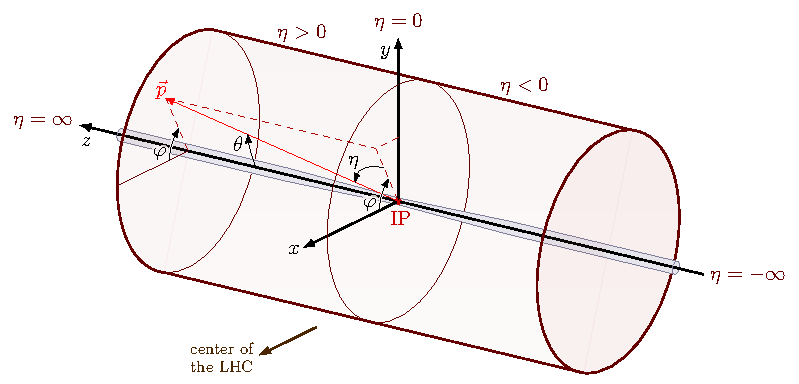
\includegraphics[width=.8\textwidth]{Figs/coords.pdf}
        \caption{Modified cylindrical coordinate system used at the LHC~\cite{coords}.}
        \label{fig:coords}
    \end{center}
\end{figure}

We place the $z$-axis along the beamline with its origin at the interaction point (IP). The IP is the point at which collisions happen, right in the center of the detector. The angle around the $z$-axis is called the azimuthal angle, denoted by $\varphi$. Sometimes in the literature $\varphi$ ranges from 0 to $2\pi$ and sometimes it ranges from $-\pi$ to $\pi$. We will try stay consistent and use the latter in this report, but we may need use the other convention at times. The angle from the $z$-axis to the $x$-$y$ plane is called the polar angle, denoted by $\theta$, and runs from 0 to $\pi$. We are interested in the standard 3-momentum of particles that we track in the detector, which we call $\vec{p}=(p_x,p_y,p_z)$, but we also define the transverse momentum as 
\begin{equation}
    p_{\mathrm{T}}=\sqrt{p_x^2 + p_y^2}.
    \label{eqn:transverse momentum}
\end{equation}
We define the rapidity, often denoted as $y$, as
\begin{equation}
    y=\frac 12 \ln\left(\frac{E+p_z}{E-p_z}\right)
    \label{eqn:rapidity}
\end{equation}
where $E$ is the total energy of the particle being considered and $p_z$ is the momentum in the $z$ direction~\cite{kar_exp_phys}. This quantity is useful as differences in rapidity are Lorentz invariant for boosts along the $z$-axis. One issue, however, is that the energy of a particle is hard to measure, so we instead use pseudorapidity, denoted as $\eta$. Rapidity and pseudorapidity are equivalent for massless particles, and near equivalent for particles with total 3-momentum magnitude $p$ much greater than their mass $m$. Pseudorapidity is much easier to measure as it is defined in \cite{kar_exp_phys} as
\begin{equation}
    \eta=-\ln\tan\frac{\theta}{2}.
    \label{eqn:pseudorapidity}
\end{equation}
From \cref{fig:coords} we see that for $z$ positive, $\eta$ is also positive, and similarly for $z$ negative. Confusingly, we define the ``forward region'' of the ALICE detector as the region for which $z$, and thus $\eta$, are negative. The forward region is where our interest lies.

The four coordinates that we use most often are $z$, $\varphi$, $p_\mathrm{T}$, and $\eta$. 

\subsection{ALICE Run 3}
In 2018, the LHC shut down for what was called Long Shutdown 2 (LS2). During this time, the ALICE experiment was being prepared for Run 3, where it will be taking data at higher energies and much higher luminosities than before, from 2022 until 2025~\cite{ALICE_Upgrade_LOI}. \Cref{fig:ALICE_Schematic} shows the detector configuration for Run 3. The intent of these upgrades was in large part to prepare ALICE for a higher luminosity of collisions in both Pb-Pb and p-p cases. 

Part of the upgrades for Run 3, the details of which can be found in \cite{ALICE_Upgrade_LOI}, were a whole new Inner Tracking System and a brand new detector called the Muon Forward Tracker. These detectors are both silicon-based and their primary purpose is tracking particles and determining the collision vertex, which is the best estimation of where the collision that resulted in these particles happened. 

The read-out electronics for many detectors were upgraded to allow for continuous read-out where necessary. The MCH also had its read-out and front-end electronics upgraded but will still work on a triggered read-out system.

\begin{figure}[h]
    \begin{center}
        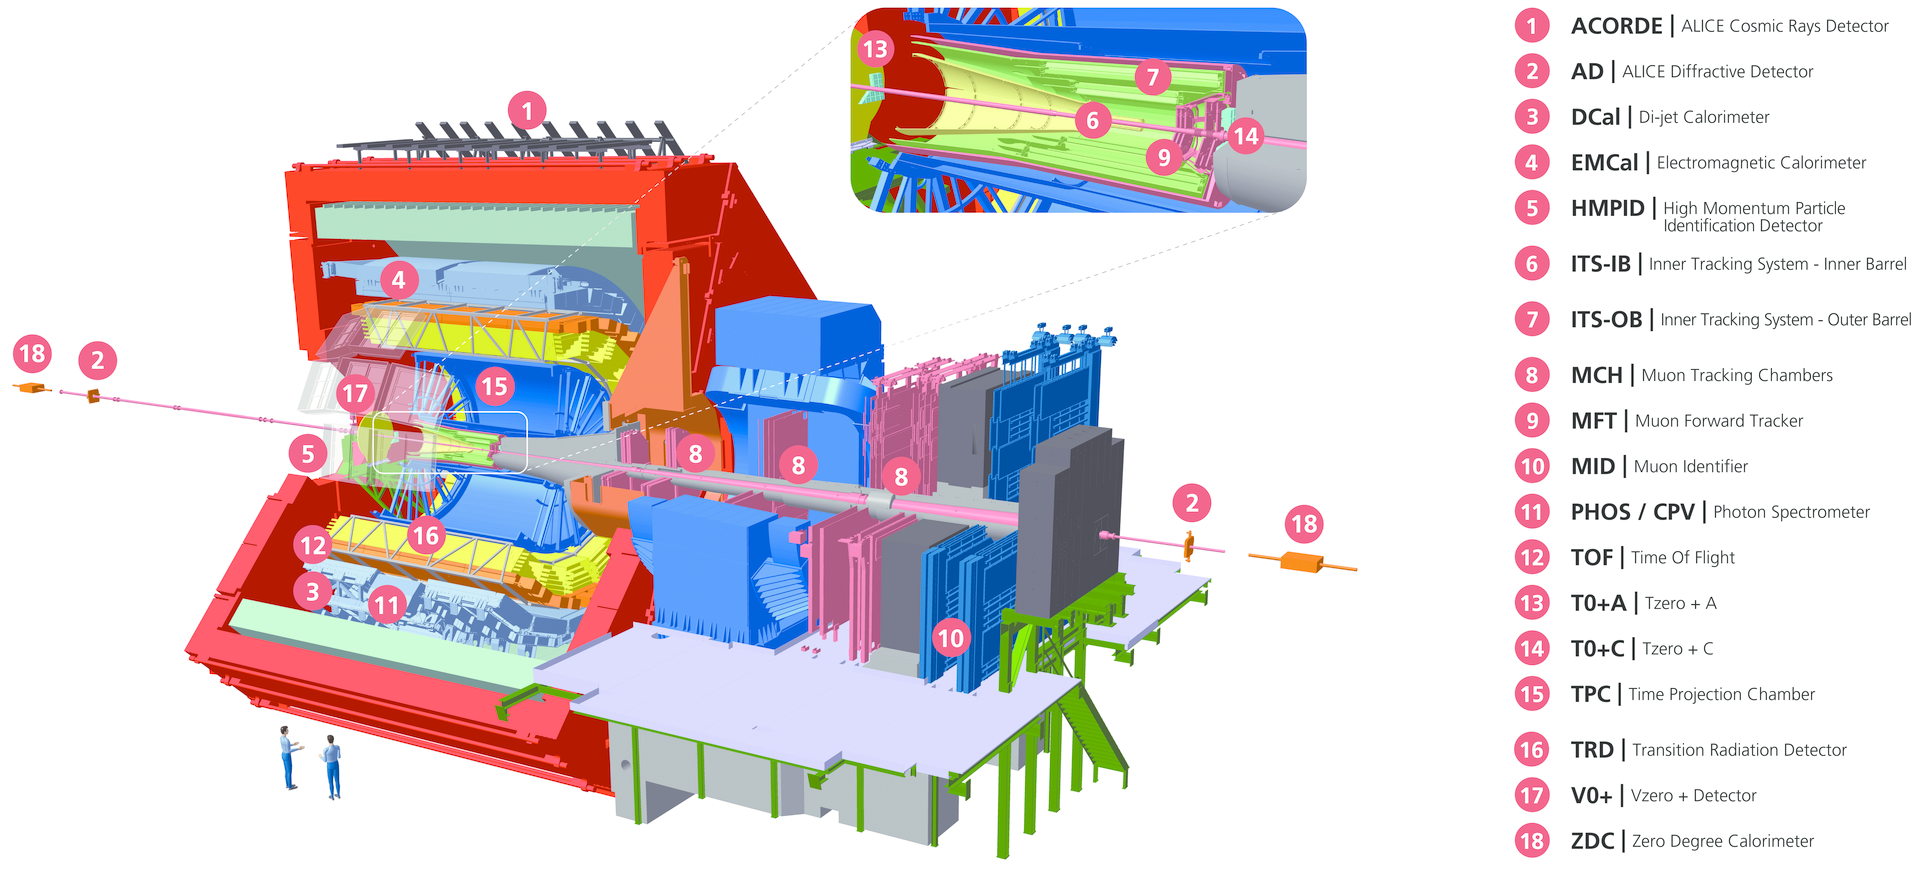
\includegraphics[width=\textwidth]{Figs/ALICE_RUN3_schematic.png}
        \caption{Schematic view of the ALICE detector setup for Run 3 of the LHC~\cite{ALICE_schematic_labels}. Note here that the MCH is shown separate from the MID, which act as the triggering mechanism for the MCH. For the purposes of this report, the MID will be considered part of the MCH. The ITS (6, 7), MCH (8), and MFT (9) are the focus of this report.}
        \label{fig:ALICE_Schematic}
    \end{center}
\end{figure}


\subsection{The Inner Tracking System}
The Inner Tracking System (ITS) sits in the main barrel of ALICE, as seen in \cref{fig:ALICE_Schematic}, and covers the range $|\eta|<1.22$~\cite{ITS_Upgrade_TDR}. For Run 3 it has been upgraded significantly by replacing the old detector with a new layout and new pixel detector technology, leading to an improvement in track position resolution at the primary vertex of a factor of 3 or greater~\cite{ITS_Upgrade_TDR}. The ITS's main purpose is to track the particles resulting from the collisions and determine the position of the primary vertex of collisions. It also serves to ``reconstruct secondary vertices, track and identify particles with low momentum, and improve the momentum and angle resolution for particles reconstructed by the Time Projection Chamber (TPC)''~\cite{ITS_Info}.

\begin{figure}[h]
    \begin{center}
        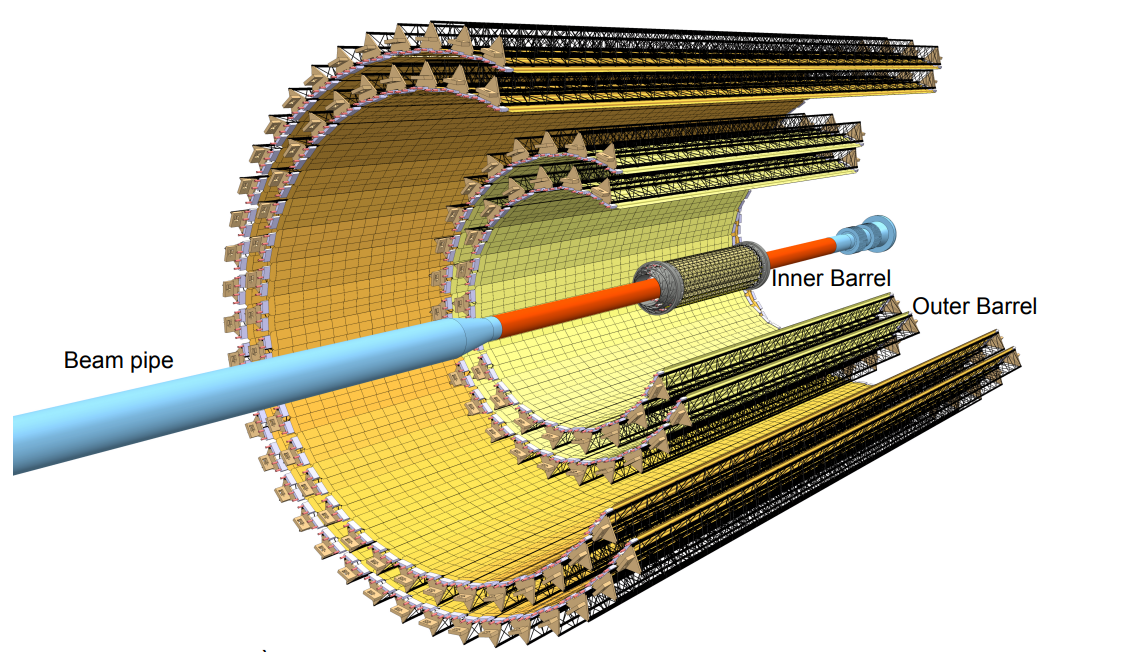
\includegraphics[width=.8\textwidth]{Figs/ITS_Schematic.png}
        \caption{Schematic view of the Inner Tracking System~\cite{ITS_Upgrade_TDR}. Note the thinner beam pipe and extremely close Inner Barrel.}
        \label{fig:ITS_Schematic}
    \end{center}
\end{figure}

The new ITS consists of 7 layers of pixel detectors; 3 in the ``Inner Barrel'' and 4 in the ``Outer Barrel''. The innermost layer sits at a radius of only \SI{22.4}{\milli\metre} from the IP thanks to a reduction in beam pipe radius for Run 3 and the outermost layer sits at a radius of \SI{391.8}{\milli\metre} from the IP. \Cref{fig:ITS_Schematic} shows the layout more clearly. 

The pixel detectors used are \SI{0.18}{\micro\metre} CMOS chips from TowerJazz. When a charged particle passes through the silicon in the active volume, it liberates the charge carriers in the material, which then collect on electrodes connected to the silicon, telling the detector that a particle has been detected. The fine segmentation of the detectors also allows the detector to determine the point at which the particle hit the detector, up to a resolution of \SI{4}{\micro\metre} in both the $r\varphi$ and $z$ directions~\cite{ITS_Upgrade_TDR}. The amount of charge deposited on the detector is dependent on the particle species and momentum (Bethe-Bloch). 

The ITS creates particle tracks in two stages. Firstly it looks at tracks found in the TPC and uses them as seeds to create tracks from the clusters of hits in the ITS with a Kalman filter~\cite{Kalman}, thus elongating the TPC tracks. This method works for particles with $\pt\gtrsim\SI{100}{\mega\electronvolt\per c}$ but below that, the TPC acceptance drops off considerably so stand-alone ITS tracking takes over, working on those clusters that were not used in the previous method. The Cellular Automaton method, described in more detail in \cref{sec:MFT_Theory}, is used for this stand-alone track finding. There doesn't appear to be a minimum number of layers required for a track to be accepted in the stand-alone regime. 

Two main methods of read-out were considered for the ITS in the new continuous read-out scheme. Firstly, a rolling shutter which continually loops through the rows of pixels and reads out the charge deposited on that pixel in the time since the last read-out was considered. The time between readings, known as the integration time, for the first method is around \SI{30}{\micro\second}. The rolling shutter scheme lends itself to needing a small number of transistors within each pixel. The second scheme is known as ALPIDE, where each pixel has a comparator that signals when the pixel has an analogue signal greater than the comparator's threshold. The signalled pixels then get read out asynchronously, according to their priority in the chain. This scheme has an effective integration time of around \SI{4}{\micro\second} but has a larger material budget. At time of writing it was not clear to us which read-out architecture is used in the ITS.

% \textcolor{red}{\textbf{\textit{NOTE THAT I AM TRYING TO FIND OUT WHICH ARCHITECTURE WAS DECIDED ON FOR THE ITS. IT'S NOT IN THE TDR AS FAR AS I CAN SEE SO IF I CAN'T FIND IT I WILL REWORK THIS SECTION A BIT}}}
% % \textbf{\textit{FIND OUT WHICH ONE WAS USED SMH}}

\subsection{The Muon Spectrometer}
The MCH sits in the forward region of ALICE, as seen in \cref{fig:ALICE_Schematic}, and covers $-4<\eta<-2.5$. It is designed to study heavy quark resonances through their single- and di-muon decay channels. As is shown in \cref{fig:Muon Spectrometer}, it is composed of a hadronic absorber, 5 tracking chambers, a dipole magnet, another absorber, and finally the 2 trigger chambers. The MFT is often also considered part of the MCH but is not shown in \cref{fig:Muon Spectrometer}. This section is adapted from the MCH Technical Design Report~\cite{MCH_TDR}.

\begin{figure}[ht]
    \begin{center}
        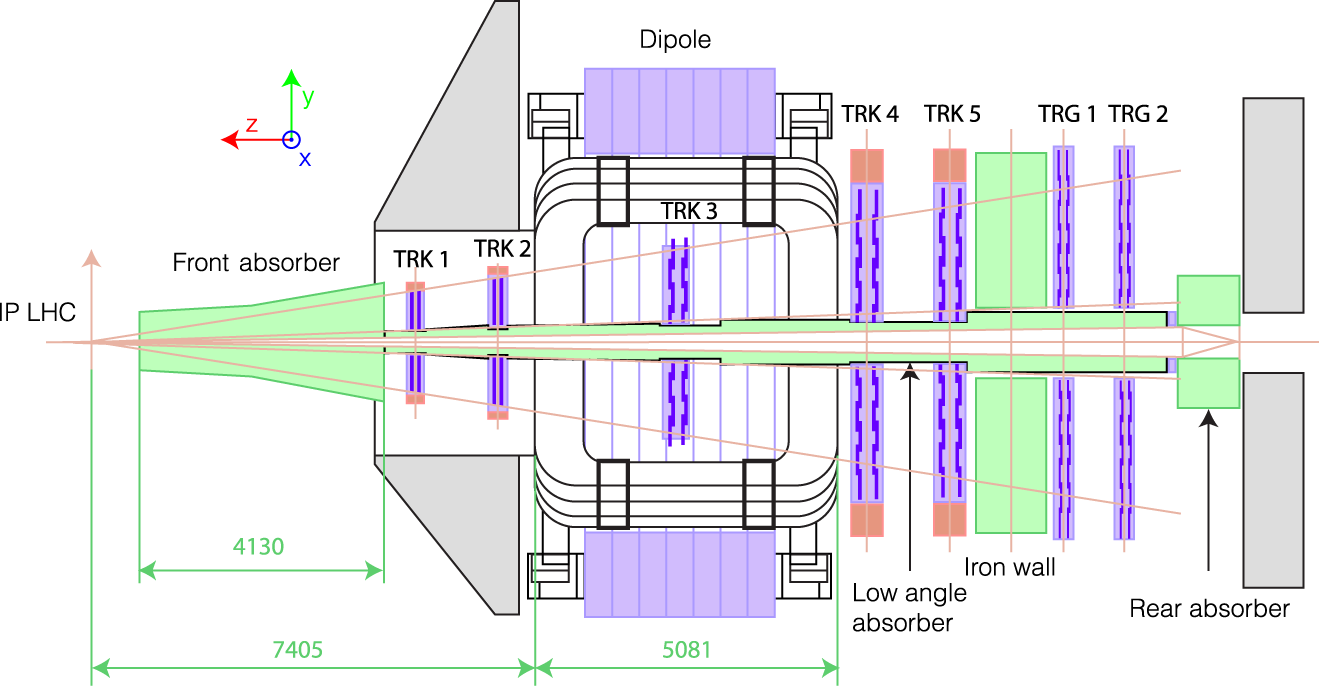
\includegraphics[width=0.8\textwidth]{Figs/MCH_schematic_pog.png}
        \caption{Diagram of the layout of the Muon Spectrometer~\cite{Muon_Spec_Schematic}. Muons pass through the absorber, are deflected by the dipole magnet, and hit the trigger chambers at the back. Importantly, all detector material sits behind the hadronic absorber, meaning the amount of data that can be used for tracking and vertexing is much lower than, say, the ITS.}
        \label{fig:Muon Spectrometer}
    \end{center}
\end{figure}

Muons don't tend to interact with matter much, especially when compared to hadrons and electrons. This makes studying muons easier, to some degree, since most other particles can be filtered out by making them pass through a large chunk of matter. As is shown in \cref{fig:Muon Spectrometer}, that is exactly what is done in the MCH. In front of any detector material (ignoring the MFT for now) sits the hadronic absorber, made primarily of carbon and concrete. This is intended to filter out all non-muon particles (mainly hadrons and photons) while not reducing the muon energy much so that they can still be studied. 

After the absorber are 5 sets of 2 cathode pad tracking detectors, situated around a large warm dipole magnet. Particles that make it through the absorber get picked up by the first two sets of detectors, then pass through the magnetic field and are deflected according to their charge, mass, and momentum. The third set tracks the particles during deflection and then the last two detect them after deflection. This set-up is particularly useful for studying di-muon events as the muons produced would be a muon-antimuon pair, which would deflect in opposite directions in the dipole magnet. This would leave a characteristic track signature that can be studied.

After the last tracking detector, particles pass through another absorber, which serves to further filter out muons from background, as well as filter out background muons. The muons produced in heavy quark resonances have considerably higher $\pt$ than those produced by background processes, so the job of the trigger system is to only trigger on muons with high enough $\pt$ to be interesting (this is defined per process) and the second absorber helps reduce the number of background muons incident on the trigger system. The trigger system is made of 2 stations of 2 Resistive Plate Chamber (RPC) detectors. Comparing the measurement of the same particle in the two stations, the $\pt$ can be determined. The decision to keep or reject an event takes about \SI{300}{\nano\second}.

In Run 1 and Run 2, the MCH performed all its own tracking and vertexing on the particles it studied. Particularly for vertexing, where the collision position is estimated, this was not optimal as most of the particles produced in the interactions didn't make it through to sensitive material. With the increased energy and luminosity of Run 3 a better system was needed to perform these tasks, so the MFT was added in front of the first absorber to take over the job.


\subsection{The Muon Forward Tracker}\label{sec:MFT_Theory}
The MFT is a brand new detector added to ALICE for Run 3 to assist the MCH with tracking and vertexing. It covers the range $-3.6<\eta<-2.45$ and was designed in conjunction with the ITS, using precisely the same CMOS pixel detectors. Due to the MFT being placed in front of the absorber, it detects a lot more particles than make it through to the MCH, allowing it to be much better at finding the primary vertex of collisions. \Cref{fig:MFT Schematic} shows the design of the MFT. The rest of this section is adapted from the MFT Technical Design Report~\cite{MFT_TDR}. 

\begin{figure}[ht]
    \begin{center}
        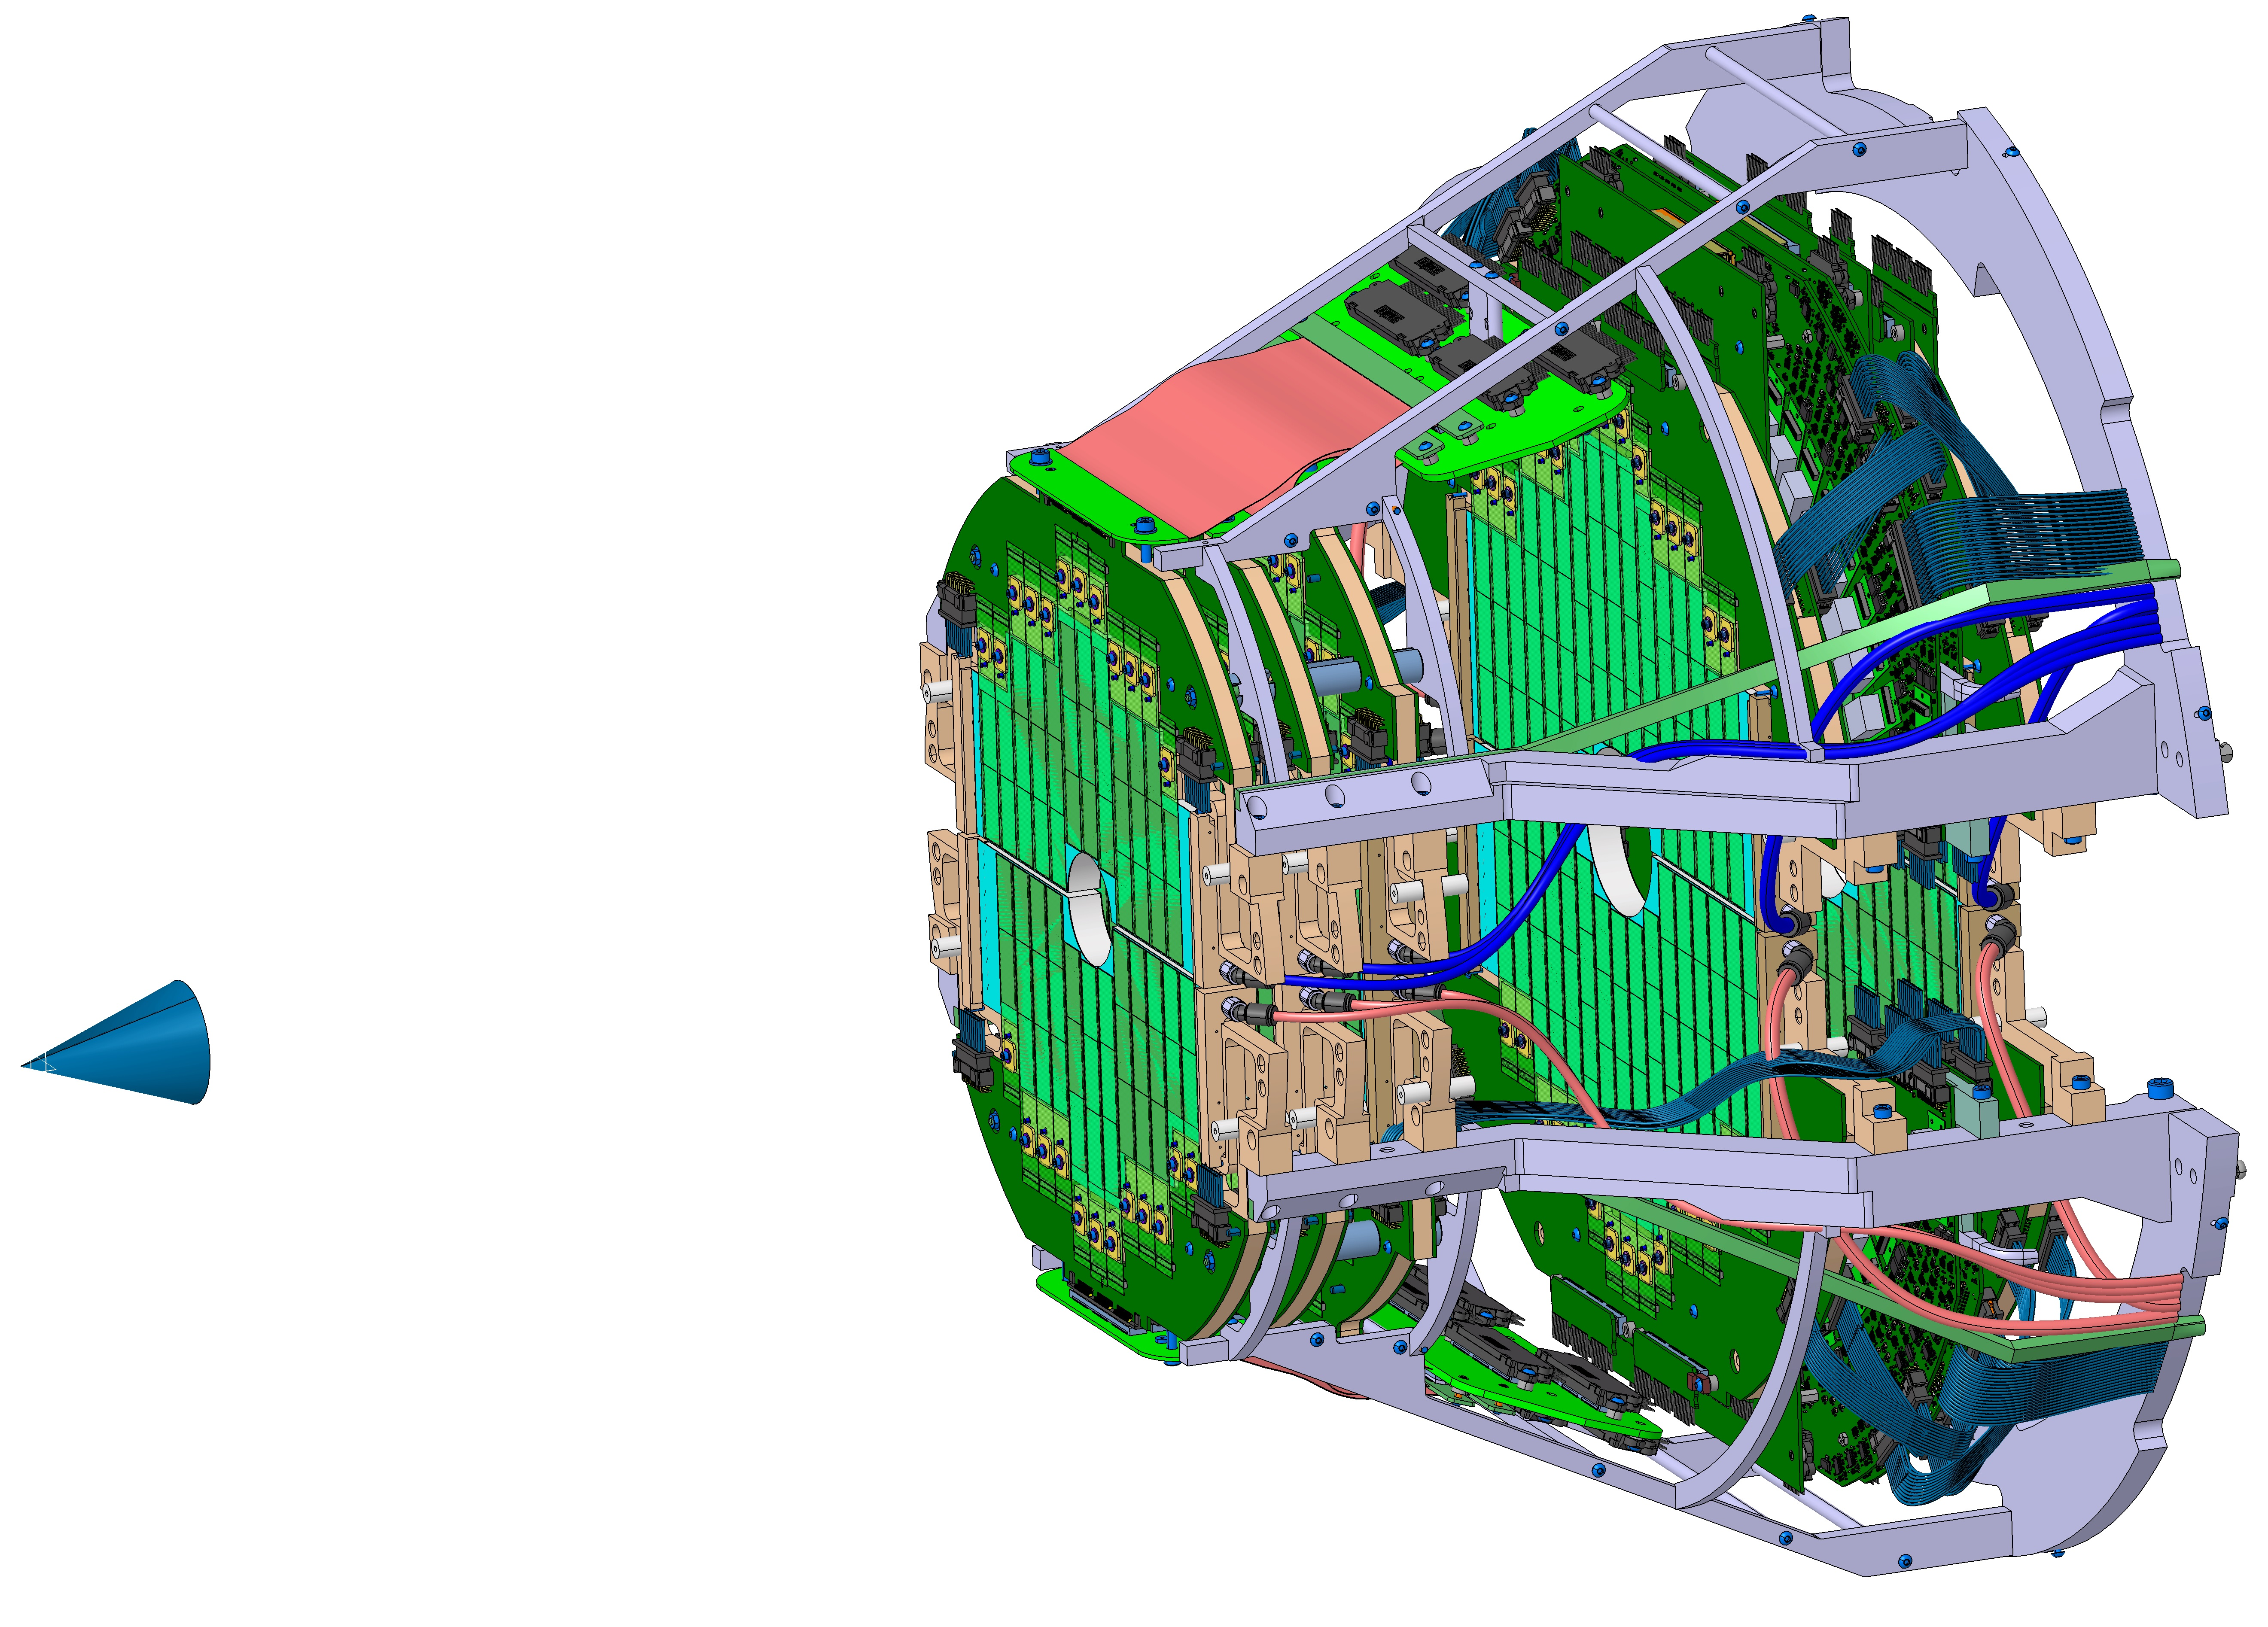
\includegraphics[width=.8\textwidth]{Figs/MFT_schematic.jpg}
        \caption{Schematic view of the Muon Forward Tracker~\cite{MFT_Schematic}. The small cone on the left shows the IP. Note that the 5 disks each have a front and back plane of pixel detectors, totalling 10 $z$-positions for the MFT to ``see'' particles at.}
        \label{fig:MFT Schematic}
    \end{center}
\end{figure}

The MFT is made of two identical half-cones sandwiching the beam pipe from above and below, each with 5 half-disks positioned at different distances from the IP along the $z$-axis. Each half-disk has a front and back detection plane totalling 10 detection planes. As the disks get further from the IP their radius increases in order to cover the same $\eta$ range, aside from the second disk, which is identical to the first. The disks sit at $z$-positions -46.0, -49.3, -53.1, -68.7, and -76.8 \si{\centi\metre} respectively and each disk is \SI{1.4}{\centi\metre} thick, leading to detector planes at $\pm \SI{0.7}{\centi\metre}$ from each of those positions.

\begin{figure}[h]
    \begin{center}
        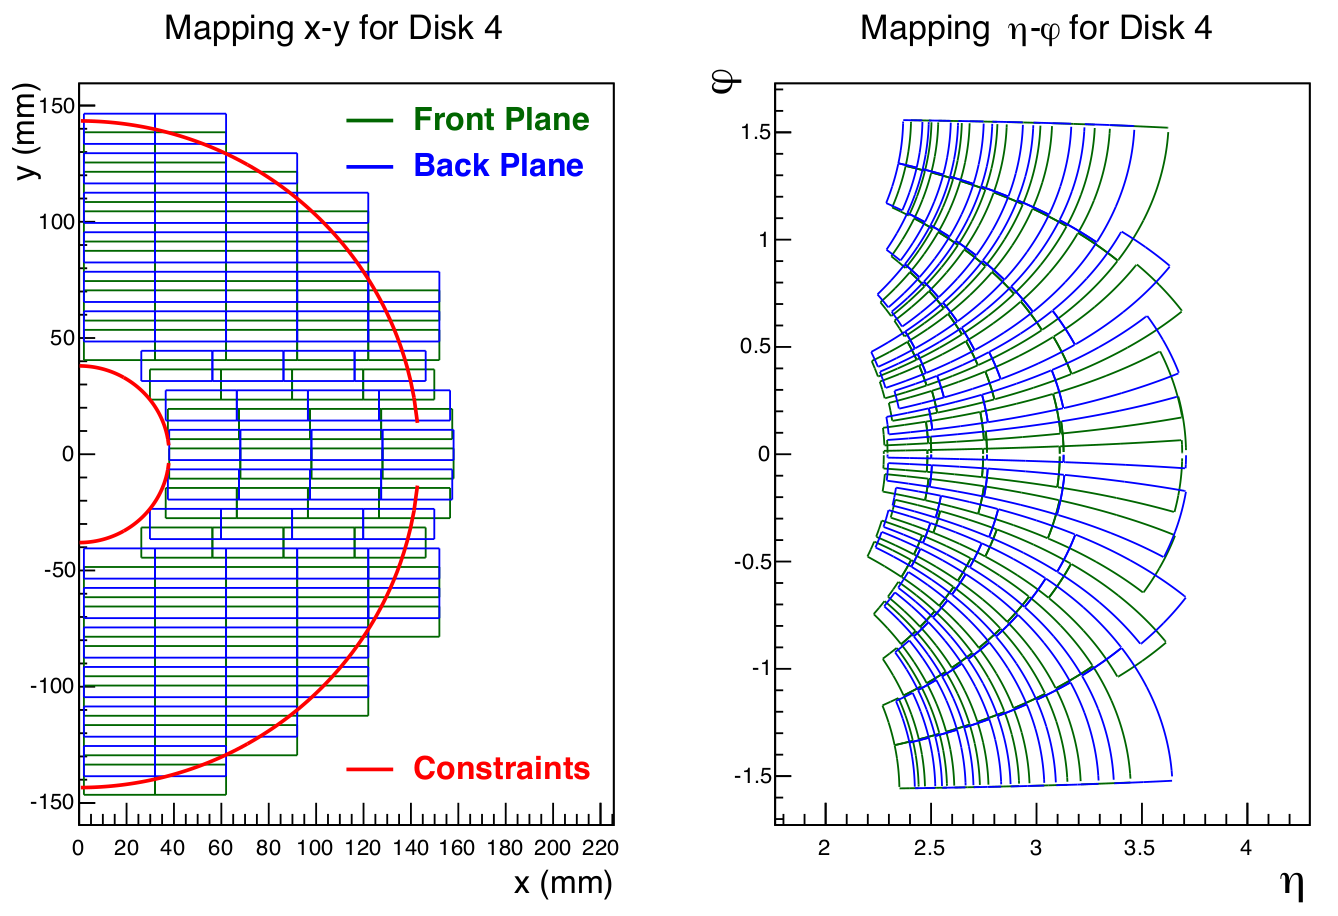
\includegraphics[width=.8\textwidth]{Figs/MFT_Disk4_mapping.png}
        \caption{The layout of pixel detector elements on the front and back plane of one of the half-disks of disk 4 in the MFT. Note that the front and back plane have layouts offset to each other by half the width of the pixel elements. This figure is taken from \cite[fig.~6.1]{MFT_TDR} but we would like to point out that the axes are labelled incorrectly in both cases; on the left, $x$ and $y$ should be swapped as the ladders run vertically and on the right $\varphi$ should run from $-\pi$ to 0 while $\eta$ should be negative.}
        \label{fig:MFT_Disk4_mapping}
    \end{center}
\end{figure}

The half-disks are made from ladders of 2 to 5 rectangular pixel detector elements. \Cref{fig:MFT_Disk4_mapping} shows an example of the layout of the front and back planes of detector elements in both $x$-$y$ and $\eta$-$\varphi$. 

The MFT performs stand-alone track reconstruction in two steps. ``Track finding'' filters through clusters (groups of hits in a certain layer) to group into track candidates and then ``track fitting'' fits tracks to those clusters and determines kinematics and covariance matrices. A Kalman filter~\cite{Kalman} is used for the track fitting but while it could also be used for the track finding, a more advanced algorithm is used to increase efficiency and reduce computation time. 

There are two algorithms used in conjunction to group clusters into track candidates. The first, called the Linear Track Finder (LTF) Algorithm, assumes that, in the $\eta$ region that the MFT occupies, the solenoid magnet surrounding the central barrel has a reduced bending effect on tracks, leading to effectively straight tracks. A ``seeding line'' is determined from clusters in the first and last disk, often with the help of the position of the primary vertex, and the algorithm simply minimises the distance of clusters to that line. There is a single parameter for this algorithm which is the radius around a cluster to allow a seeding line to be considered. While the LTF method is very computationally inexpensive, its straight line assumption breaks down at low momenta, so the Cellular Automaton (CA) algorithm is implemented to pick up the pieces.

The CA algorithm works by pairing clusters in neighbouring disks into ``cells'' and then iterating through cells and determining, based on a number of parameters such as maximum deviation angle and maximum $\theta$ angle of a cell according to the collision vertex, whether neighbouring cells are ``compatible'' and grouping those cells together as candidates for a track. This algorithm depends on having a determined position of the collision vertex to both create cells and to match cells together as in both cases they need to point towards the vertex within some pre-defined limit. This vertex position can be supplied by external means, such as the ITS, or it can be estimated using cells between the first two disks. The algorithm also has a default minimum track length in terms of number of disks involved in the process, which is set by default at 4 out of 5 disks. 

Due to the number of cluster combinations that the CA algorithm needs to consider compared to LTF, it ends up being considerably more computationally expensive to run. Since both methods have their advantages, particularly with CA picking up the slack in the low momentum (and specifically low $\pt$) regions, both methods are implemented. LTF goes first, finding as many high $\pt$ tracks as it can, and then CA runs on the clusters that the LTF did not find tracks for. This reduces the overall computation time and take advantage of both algorithms as much as possible. 


\subsection{The Online-Offline Analysis Framework}
With the increased interaction rate intended for Run 3, a new system for real-time processing, as well as offline analysis, needed to be constructed~\cite{ALICE_Upgrade_LOI}. The Online-Offline (O2) framework was developed for this purpose. This section is mostly adapted from the O2 Upgrade TDR~\cite{O2_Upgrade_TDR} as well as the O2 documentation at \url{https://aliceo2group.github.io/analysis-framework/}.

\begin{figure}[h]
    \begin{center}
        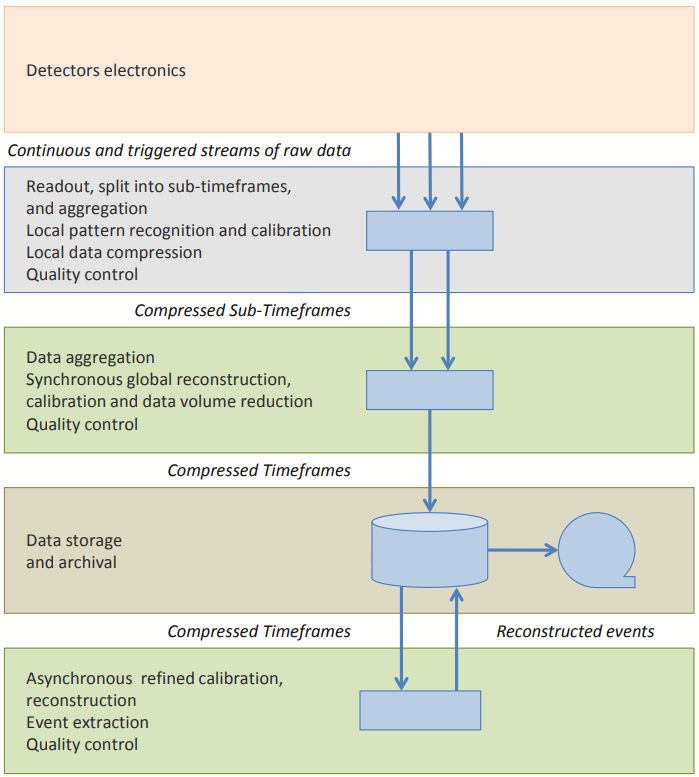
\includegraphics[width=.6\textwidth]{Figs/O2_flow.png}
        \caption{Functional flow of the O2 framework~\cite{O2_Upgrade_TDR}. Detectors output their signal continuously in the new configuration and this signal gets split into chunks called timeframes. These timeframes get processed a number of times, reducing the volume of data each time by only extracting the quantities that will be used for analysis. Many choices have to be made at each step to ensure that useful data makes it out the other side and so the details of this process are always in flux.}
        \label{fig:O2_flow}
    \end{center}
\end{figure}

\subsection{Online Analysis}
The ``Online'' portion of the framework is the part that does all the synchronous processing, i.e. as the raw data is continuously read out from the detectors. The data is first stored in ``sub-time frames'' (STFs), which get processed to generate clusters in order to reduce the volume of data and then get built into ``time frames'' (TFs) of \SI{10}{\milli\second} chunks of data. From there the data gets its first pass of detector reconstruction, e.g. track finding, and then gets compressed into ``compressed time frames'' (CTFs). The CTFs are stored on disk and that is where the Online portion ends. Note that at each step, QC and calibration data is extracted and stored for later use.

\subsection{Offline Analysis}
With the CTFs stored to disk, they can then by processed asynchronously into Event Summary Data (ESD) and then Analysis Object Data (AOD) files. ESDs are not used for analysis and are stored for a while before being deleted. AODs (real and simulated) and CTFs are the only persistent data type. 

The process of turning CTFs into AODs is called ``reconstruction'' and is often performed multiple times on the same data. Iterations of reconstruction are called reconstruction passes and these passes will usually be done many times if the previous passes missed something in their reconstruction, or perhaps if a certain table was not populated in the reconstruction but someone needs that table for their analysis. As a result of this, two different passes on the same data can end up with very different-looking results. 

We distinguish between data taken in Run 3 and data taken in Runs 1 and 2 by calling Run 3 AOD's ``AO2D'' files, and Run 1 and 2 just ``AOD'' files. The data is stored on the \OldTexttt{alimonitor} system, requiring a certificate to access, which is obtained by joining the ALICE collaboration. Access to all data and most analysis tools used in this report is restricted behind this wall. AODs can then be analysed using an ``Analysis Task'', which is written in C\OldTexttt{++} and ROOT. 





The focus of the upgraded analysis framework was to reduce disk space usage when processing and analysing, as well as making sure all analysis takes advantage of all processing power available to it at all times.